
\section{Generative Models and Large Language Models}

A recent trend, one that has gained notoriety in circles far outside of machine learning, is the usage of generative AI
or large language models \textit{LLMs} for both ML and non-ML applications. These are largely unsupervised, or sometimes
semi-supervised, algorithms that generate content from analyzing existing content. This content is often text, but in recent
multi-modal models such as OpenAI's GPT-4\cite{openai2023gpt4}, can be other modalities such as images as well, or even a combination thereof.

Large Language Models have gained traction specifically because they have arguably reached human-level performance, and according
to some even passed it, on various tasks of generating text. The word "large" here is an understatement,
as these models have billions upon billions of parameters, and rely on neural architectures that stack transformers and other large
computational operations across many GPUs. They are trained on massive amounts of text, sometimes on the order of trillions\cite{touvron2023llama} of tokens.

What makes these newer language models such as OpenAI's \textit{ChatGPT}, Meta AI's \textit{Llama}\cite{touvron2023llama}, or Google's \textit{Bard} so special is their ability to generalize to new tasks \textit{without any fine-tuning or training}.
What this means is that we can simply provide an instruction (also called a \textit{prompt}) to the model, and it will generate text that is consistent with it.
Moreover, these models are exhibiting remarkable emergent abilities, meaning things they were never explicitly trained on.
These include common sense reasoning, the ability to use tools (e.g. search, calculator, write and execute code, invoke APIs etc.), and even theory of mind (e.g. understanding that other agents have their own beliefs, desires, and intentions)\cite{bubeck2023sparks,openai2023gpt4}.

As it turns out, the key to unlocking these abilities lies in an elaborate fine-tuning process after extensive pre-training on a large corpus of text.
In the case of ChatGPT, this was done in a novel way using a method called Reinforcement Learning with Human Feedback \textit{RLHF} targeted iteratively improving the model by specifically
rewarding high-quality content and penalizing toxic feedback.\cite{ouyang2022training} Because these models are trained on text across the internet, which
unsurprisingly included troves of nonsense and hate speech, these models must be pushed away from purely unchecked generation of content,
as this can be dangerous. While the possibility of generating this text can never be fully eliminated, or can perhaps be circumvented with the right prompts, it remains true that this can be controlled as we add more human feedback.

One big remaining challenge is to control the tendency of these models to hallucinate, meaning they make up facts that are not true or not provided in the context, while sounding very confident and authoritative.
You should never trust the output of a LLM unchecked, especially when providing medical advice or making other critical decisions.
They can still be very useful if used with caution and in the right context to save enormous amounts of time and effort.

\subsection{Instruction Tuning}

“Instruction tuning” refers to fine tuning a language model of NLP tasks described with instructions, often with the aim of having the model
be able to perform admirably on tasks on which it was never trained. Let's take a look at an example.

Consider the Google FLAN\cite{chung2022scaling} model. As illustrated in figure 2.13, this model was provided not only a variety of datasets, but
tuned with a variety of different tasks. Instructions were provided for the model to reason through many types of question answering, but also text
generation tasks, common-sense reasoning tasks, or even tasks related to program execution. Researchers found that by fine-tuning a variety of instruction
sets in this manner, models are able to generalize to not only these types of task but other tasks as well.

\begin{figure}
  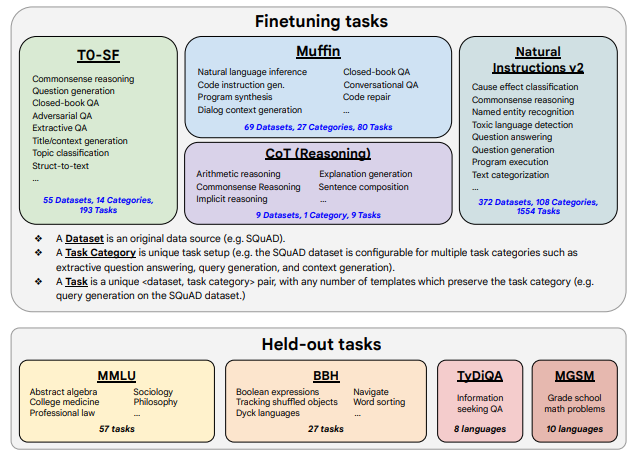
\includegraphics[width=\linewidth]{chapters/NLP/figures/flan_finetune.png}
  \caption{This figure, taken from the original Google FLAN paper, illustrates a model that was fine-tuned using a variety of instruction prompts, and tested using a set of held out instruction.}
  \label{fig:flan_instruction_fine_tuning}
\end{figure}

This is a powerful step in the field of Artificial Intelligence. A model receiving instructions on common-sense reasoning tasks generalizing to an ability to perform tasks like arithmetic is a step
toward generalized intelligence in AI systems. If enough of these types of prompts are instruction sets related to medical tasks, would a model be able to generalize to other types of information in the field?

\subsection{LLMs in Medicine}
\textbf{DISCLAIMER:} Generative Language Models, while extremely powerful, should never solely be relied upon for medical advice. The examples in this text,
as well as the models that are referenced, are used purely for educational purposes only.
These models are growing at rapid pace, and this trend will very likely continue in the coming years. As they become more powerful, there
will inevitably be questions as to how they can be used within the medical field. Remember that an AI is trained on reading the text on the internet,
a haven for misinformation, and this should give you all you need to know that they should never be used to make a decision about a patient. What might be more dangerous than this
misinformation is the tendency for these types of models to \textit{hallucinate}, a term that refers to these models generating sequences that are inconsistent with their training data.
What makes these particularly dangerous is that these hallucinated sequences are often confident responses.

That being said, that does not mean they are not useful. Consider the task in the previous section where we identified whether or not a piece of text
expressed a difficulty in attaining or maintaining employment. This is the sort of task that an LLM can also help with. All we have to do
is design a prompt that lets the LLM know what we are trying to model and provide the text sample.

\subsection{Public vs Private Models}

Can we simply send patient data, or even survey responses, to ChatGPT and ask for results? Of course not. ChatGPT is a model owned by OpenAI we cannot send
patient data over an API. However, there are LLMs with weights that can be downloaded and used on a local machine, or within the compute plane of a healthcare
organization. In all likelihood there will be more LLMs to come that are specialized to medicine that can be used as well. If you download one of these models,
it is no different than using any other machine learning model.

It is worth noting that there are likely to be state and national regulations surrounding the use of AI models, particularly LLMs, with respect to user data, and
that as they develop we make sure to be in compliance.

\subsection{Epilepsy Example}

Consider the following example output from a state-of-the-art unnamed LLM that targets the task from the previous section.

First let's try the sample positive:

\begin{displayquote}
  \textbf{Prompt:} Does the following quote express a person's financial difficulties in their ability to maintain or attain employment: "We have found that employers are far less likely to want to hire our son because of his condition."
\end{displayquote}

\begin{displayquote}
  \textbf{LLM Response:} LLM: Yes, the quote suggests that the parents of a child with a disability are saying that employers are less likely to want to hire their son due to his condition. This could have a significant financial impact on the person's ability to attain or maintain employment.
\end{displayquote}

It looks like the LLM got this example correct. And now we can try the sample negative:

\begin{displayquote}
  \textbf{Prompt:} Does the following quote express a person's financial difficulties in their ability to maintain or attain employment: "The medication costs are through the roof and it is simply too much for us to be able to handle."
\end{displayquote}

\begin{displayquote}
  \textbf{LLM Response:} Yes, the quote suggests that the person is struggling to afford the cost of their epilepsy medication. This could have a significant financial impact on their ability to maintain or attain employment.
\end{displayquote}

Notice that this example is incorrect, though the reasoning is sound. This illustrates an important point in the usage of LLMs, and that is Prompt Design

\subsection{Prompt Engineering}

Prompt design is key to the success of LLMs. In the above example, the model believes that the cost of epilepsy medication itself may lead to a difficulty in maintaining or attaining a job. While this might be true, the target was a direct expression of this difficulty.
If we modify the query to express this directly, we get the kind of result we were looking for, at least in this case:

\begin{displayquote}
  \textbf{Prompt:} Does the following quote discuss the difficulty in maintaining or attaining employment: "The medication costs are through the roof and it is simply too much for us to be able to handle."
\end{displayquote}

\begin{displayquote}
  \textbf{LLM Response:} No, the statement you provided does not specifically discuss the difficulty in maintaining or attaining employment. It focuses on the high cost of medication and how it's difficult for the person making the statement to handle it.
\end{displayquote}

Keep in mind that when working with LLMs, iterating on your prompts is well worth your time. You should work to clearly express what you are trying to solve.

Some of these models have larger context lengths than others. What this means is that they can handle more input tokens, such as a longer set of instructions, or in our case a longer quote.
You should try to use a model that can fit the entire context of the task at hand.

\subsection{Fine-Tuning}

It is very likely that models will soon be fine-tuned to the medical domain. What this means is that they tradeoff accuracy in their abilities to answer general prompts for an increased accuracy in their ability to answer prompts related to a target.
In the same way that a transformer model like RoBERTa was fine-tuned to our task in the previous section, an LLM can have their weights fine-tuned.
Currently, LLM fine-tuning to specific tasks comes at prohibitive costs. However, LoRA\cite{hu2021lora} optimization techniques are the method most often used to combat these costs. They inject trainable decomposed matrices into the transformer architectures that
are easier to train than the entire model, which may be extremely large.
This is beyond the scope of the current chapter, but these tools will soon become common place and it is not beyond the realm of possibility for a model to be fine-tuned specifically to deal with
epilepsy.

\subsection{What Comes Next}

The development of LLMs will continue in the years to come. At the time of this text, Artificial Intelligence with respect to NLP is growing as fast as it ever has, and the general public is becoming more aware of their abilities. Above all else, we
must remain vigilant with respect to privacy concerns, bad actors, and the understanding that these models should not be used for medical advice.

It is likely that we will be able to fine-tune them, say on EHRs, for a series of questions relating to retrospective research. Until then, monitor the regulations around LLMs as well as the tools and frameworks created by researchers and engineers in the field.
